\documentclass[a4paper]{article}
\usepackage{fullpage}
\usepackage[top=0.5in, bottom=0.5in, left=0.5in, right=0.5in]{geometry}
\usepackage{hyperref}
\usepackage{lettrine}
\usepackage{color}
\usepackage{array}
\usepackage{tabu}
\usepackage{float}
\usepackage{graphicx}
\usepackage{cite}
\hypersetup{colorlinks=true,linkcolor=blue,urlcolor=blue}
\usepackage{type1cm} % scalable fonts
\begin{document}
\title{A Practical Guide To Analyze Data from the SRBC Water Quality Monitoring}
\author{Eswara Sravani Munnangi, Joss C.Steward and Dr. Jeonghwa Lee}
\date{\vspace{-2ex}}
\maketitle
\begin{minipage}[t]{0.45\textwidth}
{\normalsize\textit{\textbf{ Abstract---}}}{
  \normalsize 
  \textbf{Today more data will be gathered and processed than ever before. This is the age of Big Data. However, with huge amounts of data comes huge performance issues. Although many performance problems can be solved simply by throwing more computing power at them, we Wish to solve these problems through software optimization instead of hardware improvements.We propose a research project focused on allowing rapid access to large amounts of data on subpar hardware. Our project will focus on the e-client storage and rapid retrieval of infrequently accessed data.}}
\definecolor{darkblue}{rgb}{0,0,0.5}
{\normalsize \textit{\textbf{\\Website---}}}\url{http://www.srbc.cs.ship.edu}
\section*{INTRODUCTION}{\normalsize 
The sample data for this project will come from the real world. 
We have decided to use water-quality information gathered by the Susquehanna River Basin Commission and made available to the public through their web site. 
At the current time, the Susquehanna River Basin Commission (SRBC) provides free access to water quality data gathered prior to December 31, 2011. 
For data gathered after December 31, 2011 there is a charge of \dollar{250} per quarter of data. Because of this fee, we will be using data gathered before December 31, 2011 for the foreseeable future.
Presumably, the SRBC does not have the resources to monitor all the stations all the time. 
Each sample contains the following information: Water Temperature, Specific Conductivity, PH level, Turbidity, and Dissolved Oxygen Content. 
Each sample also includes metadata consisting of a Time Stamp and the Station Name. }
\renewcommand\footnoterule{\rule{\linewidth}{0.5pt}}
\footnotetext{ {\footnotesize Manuscript received June xx, xxxx: revised June xx, xxxx. This work was supported in part by xxx. 
\begin{description}
  \item[$\bullet$ ] Eswara Sravani Munnangi is with the Department of Computer Science and Engineering, Shippensburg University, Shippensburg, PA 17257,(\email{em8678@ship.edu}).
  \item[$\bullet$ ] Joss C. Steward is with the Department of Computer Science and Engineering, Shippensburg University, Shippensburg, PA 17257, (\email{js0289@ship.edu}).
   \item[$\bullet$ ] Dr. Jeonghwa Lee is with the Department of Computer Science and Engineering, Shippensburg University, Shippensburg, PA 17257, 
     Please address any correspondence to Dr. Jeonghwa Lee - \url{http://www.cs.ship.edu/~jlee} (\email{jlee@ship.edu}).
\end{description}}}
\end{minipage}  
\hspace{.5cm}
\begin{minipage}[t]{0.45\textwidth}
{\normalsize  
A quick glance at the data gathered in Q1 of 2010 reveals that the SRBC has been gathering water-quality data from 60 stations. 
The sample rate seems to vary between stations from once every 5 seconds to once every 4 hours. 
This is not actually an overwhelming amount of data. 
Assuming one sample every 5 seconds, each station would produce approximately 6,307,200 samples per year. 
Given 60 stations, that would be 378,432,000 samples per year. 
This may seem like a lot, but given that the largest Microsoft SQL Server databases in 2008 were exceeding 1 petabyte in size adding fewer than 400 million rows per year is completely feasible. 
However, it should be obvious that not every organization capable of producing data on this scale can afford to run server farms powerful enough to process and store this much data. 
Ideally, we will be able to store all of the data collected and still be able to access it in reasonable amounts of time on relatively low end hardware. 
To accurately gauge performance, we will store the data in a indexed SQL Server database and compare the resulting size and performance to any other data storage schemes we come up with. 
Other possibilities include storing infrequently accessed data in segmented compressed files and storing statistics such as min, max, standard deviation, and etc. on each compressed segment of data in a SQL Server Database. 
The overall performance may prove to be satisfactory using existing software and standard techniques. 
If that is the case, we will still attempt to achieve a performance gain through the use of special techniques. 
Our hope is that this study will aid in the storage and analysis of large amounts of data on slower, more power efficient hardware than is currently required.}
\section*{OVERVIEW}{\normalsize 
The Susquehanna River Basin Commission (SRBC) initiated the establishment of the Remote Water Quality Monitoring Network (RWQMN) in January 2010.
The main objective of this Monitoring Network (RWQMN) is to continuously monitor the conditions of rivers and streams located in Northern Tier region of Pennsylvania and Southern Tier region of New York, producing periodic reports on the water quality for use by Susuquehanna River Basin Commission (SRBC) officials. 
Ideally, this system could also provide rapid alerts, warning officials of water quality issues in real time.}
\end{minipage}  
\newpage
\begin{minipage}[t]{0.45\textwidth}
\section*{\small Stations}
{\normalsize  The stations are operating in areas where drilling for natural gas is most active, as well as other locations where no drilling activities are planned so SRBC can collect control-data. A contribution from East Resources provided the initial funding for the project. In 2010, the New York State Energy Research and Development Authority provided funding for the expansion of the network into the New York portion of the basin. SRBC is covering the ongoing maintenance costs. \par
The monitoring network provides constant data collection with instruments sensitive enough to detect subtle changes in water quality on a frequency that will allow background conditions and any changes to them to be documented throughout the year. The following five water quality parameters are being measured at each station:
\begin{description}
  \item[$\bullet$ ] Water Temperature
  \item[$\bullet$ ] pH
  \item[$\bullet$ ] Specific Conductance
  \item[$\bullet$ ] Dissolved Oxygen
  \item[$\bullet$ ] Turbidity
\end{description}
}
\section*{\small Water Temperature}
{\normalsize Water temperature is very important to fish and other aquatic life, as well as for swimmers, fishermen, and industries. Temperature affects the ability of water to hold oxygen, which can affect respiration and an organism's ability to resist certain pollutants. Human induced changes to water temperatures can have a great effect on stream ecosystems. The loss of riparian tree cover can raise stream temperatures through exposure to the sun. In addition, a lot of water in the Susquehanna Watershed is used for cooling purposes in power plants that generate electricity, resulting in warmer water releases back to the environment. The temperature of the released water can affect downstream habitats.}
\section*{\small pH}
{\normalsize pH is a measure of water's acidity/basicity. The range goes from 0 - 14, with 7 being neutral. A pH of less than 7 indicates acidity, whereas a pH of greater than 7 indicates basicity. pH is really a measure of the relative amount of free hydrogen and hydroxyl ions in the water. Water that has more free hydrogen ions is acidic, whereas water that has more free hydroxyl ions is basic. Since pH can be affected by chemicals in the water, pH is an important indicator of water that is changing chemically. pH is reported in "logarithmic units," like the Richter scale which measures earthquakes. Each number represents a 10-fold change in the acidity/basicity of the water. Water with a pH of 5 is ten times more acidic than water having a pH of six. }
\end{minipage}  
\hspace{.5cm}
\begin{minipage}[t]{0.45\textwidth}
{\normalsize Pollution can change a stream's pH, which in turn can harm animals and plants living in the water.For instance, water coming out of an abandoned coal mine can have a PH of 2, which is very acidic and would definitely affect any fish's health. By using the logarithm scale, this mine-drainage water would be 100,000 times more acidic than neutral water -- so stay out of abandoned mines.}
\section*{\small Specific Conductance}
{\normalsize Specific conductance is a measure of the ability of water to conduct an electrical current. It is highly dependent on the amount of dissolved solids (such as salt) in the water. Pure water, such as distilled water, will have a very low specific conductance, and sea water will have a high specific conductance. Rainwater often dissolves airborne gasses and airborne dust while it is in the air, and thus often has a higher specific conductance than distilled water. Specific conductance is an important water-quality measurement because it gives a good idea of the amount of dissolved material in the water.\\ \par
High specific conductance indicates high dissolved-solids concentration; dissolved solids can affect aquatic life, as well as the suitability of water for domestic, industrial, and agricultural uses. At higher levels, drinking water may have an unpleasant taste or odor or may even cause gastrointestinal distress. Additionally, high dissolved-solids concentration can cause deterioration of plumbing fixtures and appliances. Relatively expensive water-treatment processes, such as reverse osmosis, are needed to remove excessive dissolved solids from water.}
\section*{\small Dissolved Oxygen}
{\normalsize A relative measure of amount of oxygen that is dissolved in given medium. Oxygen dissolved in the lakes, rivers, and oceans is crucial for the aquatic organisms and creatures living in it.
As the amount of dissolved oxygen drops below normal levels in water bodies, the water quality is harmed and creatures begin to die off. Indeed, a water body can "die", a process called eutrophication.\\ \par
A small amount of oxygen, up to about ten molecules of oxygen per million of water, is actually dissolved in water. This dissolved oxygen is breathed by fish and zooplankton and is needed by them to survive.\\ \par
Rapidly moving water, such as in a mountain stream or large river, tends to contain a lot of dissolved oxygen, while stagnant water contains little. Bacteria in water can consume oxygen as organic matter decays. Thus, excess organic material in our lakes and rivers can cause an oxygen-deficient situation to occur. Aquatic life can have a hard time in stagnant water that has a lot of rotting, organic material in it, especially in summer, when dissolved-oxygen levels are at a seasonal low.}
\end{minipage}  
\newpage
\begin{minipage}[t]{0.45\textwidth}
\section*{\small Turbidity}
{\normalsize Turbidity is the amount of particulate matter that is suspended in water. Turbidity monitors measure the scattering effect that suspended solids have on light: the higher the intensity of scattered light, the higher the turbidity. Material that causes water to be turbid includes:
\begin{description}
  \item[$\bullet$ ] clay
  \item[$\bullet$ ] silt
  \item[$\bullet$ ] finely divided organic and inorganic matter
  \item[$\bullet$ ] soluble colored organic compounds
  \item[$\bullet$ ] plankton
  \item[$\bullet$ ] microscopic organisms
\end{description} 
Turbidity makes the water cloudy or opaque, and is reported in nephelometric turbidity units (NTU). During periods of low flow (base flow), many rivers are a clear green color, and turbidities are low, usually less than 10 NTU. During a rainstorm, particles from the surrounding land are washed into the river making the water a muddy brown color, indicating water that has higher turbidity values. Also, during high flows, water velocities are faster and water volumes are higher, which can more easily stir up and suspend material from the stream bed, causing higher turbidities.\\ \par
The picture with the three glass vials shows turbidity standards of 5, 50, and 500 NTUs. Once the meter is calibrated to correctly read these standards, the turbidity of a water sample can be taken. Turbidity can be measured in the laboratory and also on-site in the river. A handheld turbidity meter (left-side picture) measures turbidity of a water sample. The meter is calibrated using standard samples from the meter manufacturer. The picture with the three glass vials shows turbidity standards of 5, 50, and 500 NTUs. Once the meter is calibrated to correctly read these standards, the turbidity of a water sample can be taken. State-of-the-art turbidity meters (left-side picture) are beginning to be installed in rivers to provide an instantaneous turbidity reading. The right-side picture shows a close-up of the meter. The large tube is the turbidity sensor; it reads turbidity in the river by shining a light into the water and reading how much light is reflected back to the sensor. The smaller tube contains a conductivity sensor to measure electrical conductance of the water, which is strongly influenced by dissolved solids (the two holes) and a temperature gauge (the metal rod).}
\end{minipage}
\hspace{.5cm}
\begin{minipage}[t]{0.45\textwidth}
\section*{DataBase Design}
Database contains two tables named
\subsection{WaterQualityData}
 Contains the following fields
\begin{center}
\begin{tabu} { | c | c | c | }
\hline
{\scriptsize Column Name} & {\scriptsize Data Type} & {\scriptsize Description }\\
\hline
{\scriptsize ID} & {\scriptsize Bigint } &{ } \\
\hline
{\scriptsize StationID} & {\scriptsize Int} & {\scriptsize Stores the station ID} \\
\hline
{\scriptsize Sample Time} & {\scriptsize Date Time} & {\scriptsize Stores the time}  \\
\hline
{\scriptsize Temperature} & {\scriptsize Float} & {\scriptsize Store the temperate value} \\
\hline
{\scriptsize Specific Conductivity} & {\scriptsize Float} & {\scriptsize Stores the specific conductivity value}\\
\hline
{\scriptsize pH} & {\scriptsize Float} & {\scriptsize Stores the pH value} \\
\hline
{\scriptsize Turbidity} & {\scriptsize Float} & {\scriptsize Stores the turbidity value} \\
\hline
{\scriptsize Dissolved Oxygen} & {\scriptsize Float} & {\scriptsize Stores the Dissolved Oxygen Value} \\
\hline
\end{tabu}
\end{center}
\subsection{Station Metadata} 
 Contains the following fields
\begin{center}
\begin{tabu} { | c | c | p{5cm} |}
\hline
{\scriptsize Column Name} & {\scriptsize Data Type} & {\scriptsize Description }\\
\hline
{\scriptsize ID} & {\scriptsize Bigint } &{ } \\
\hline
{\scriptsize Station Name} & {\scriptsize char} & {\scriptsize Stores the station name} \\
\hline
{\scriptsize Sample Location} & {\scriptsize Geography} & {\scriptsize Stores Latitude and Longitude of the station}  \\
\hline
\end{tabu}
\end{center}
\section*{Schema Diagram}
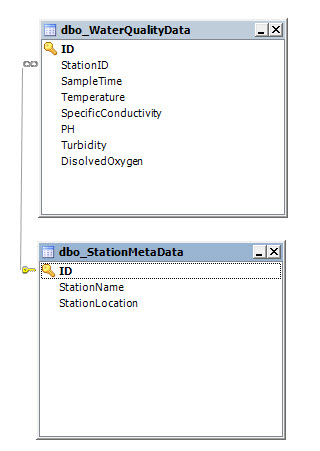
\includegraphics{schema.jpg}
\end{minipage}
\newpage
\section*{GRAPHICAL USER INTERFACE (GUI):}
The tool is very user friendly and intuitive and uses a GUI interface implemented in Aspx to communicate with the user. Various features are self explanatory.
Forms are easy to fill in and components can be added, removed and updated very easily through a single dialog box.\par List boxes are used to display all the components at once so that user can see all the components of a particular type at once. One can just select the component and modify and remove the component.
\begin{center}
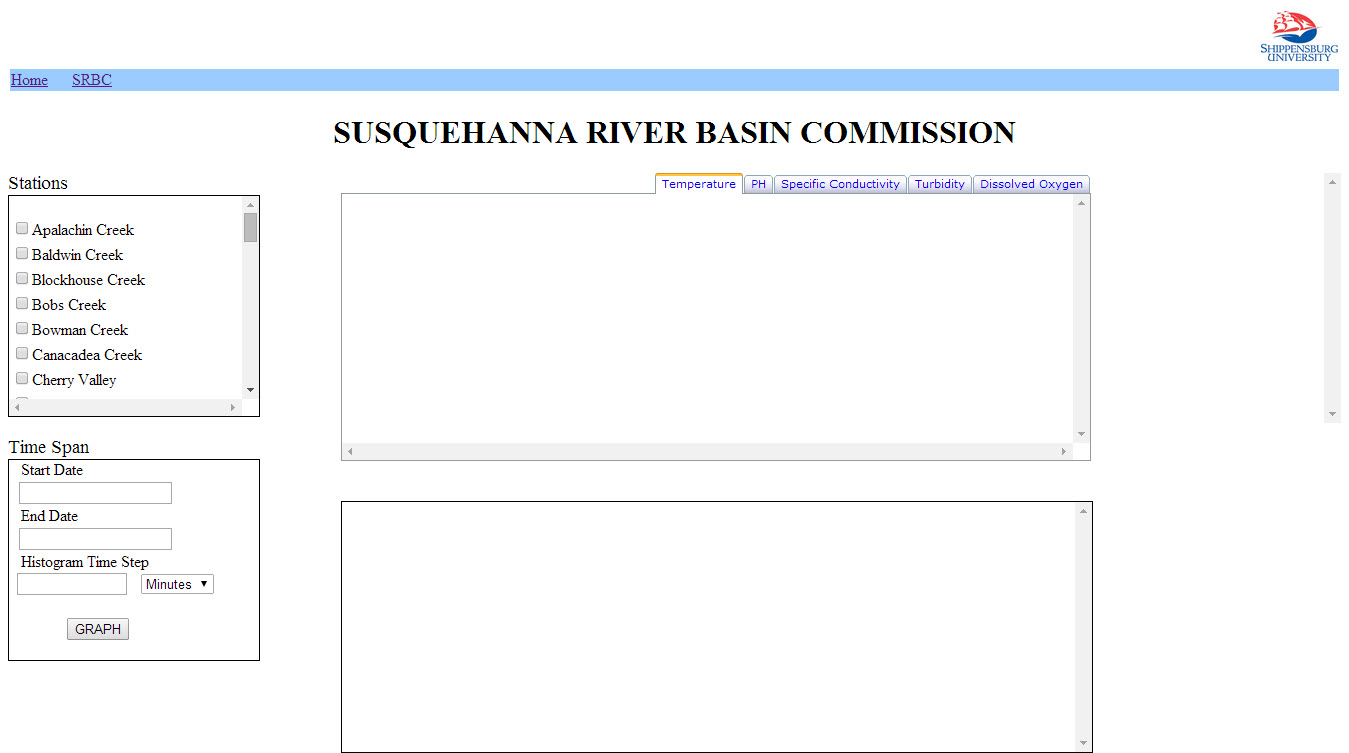
\includegraphics[scale=0.50]{srbcfull.jpg}
\end{center}
\bigskip
\bigskip
\subsection*{1. Stations Panel}
\begin{center}
\includegraphics {image3.jpg}
\end{center}
{\normalsize This panel is an Checkbox list which is used to select multiple Stations to monitor the data.}
\subsection*{2. Time Span Panel} 
\begin{center}
\includegraphics {image2.jpg}
\end{center}
{\normalsize This panel is used to select the date range for the graph to be plotted.\par Start Date textbox and End Date text box is an Ajax Calender popout textbox which enables us to select the date from the calendar in the format MM/DD/YYYY}
\begin{center}
\includegraphics {image5.jpg}
\end{center}
{\normalsize Histogram Time step is a parameter which will enable us to plot the graph by grouping the data specified in the time step intervals.}
\begin{center}
\includegraphics {image6.jpg}
\end{center}
{\normalsize Time step can be selected from any of the parameters from the dropdown list.}
\subsection*{3.Graph Panel}
\begin{center}
\includegraphics[scale=0.75] {image1.jpg}
\end{center}
{\normalsize This panel is an Ajax Tabbed Container which allows to display only one panel at a time.\\
Monitoring Parameters are listed for tabs.}
\bigskip
\begin{center}
\includegraphics[scale=0.75] {image4.jpg}
\end{center}
{\normalsize Monitoring Parameters can be any of the following
\begin{description}
  \item[$\bullet$ ] Water Temperature
  \item[$\bullet$ ] pH
   \item[$\bullet$ ] Specific Conductance
   \item[$\bullet$ ] Turbidity
   \item[$\bullet$ ]  Dissolved Oxygen
\end{description}
Expalanation about the parameters is detailed in section Overview.
}
\subsection*{4. Analysis Panel}
{\normalsize This panel is populated with the statistics data once graph is generated for better analysis.}
\begin{center}
\includegraphics{analysis.jpg}
\end{center}
\subsection*{A snapshot of the analysis for two stations:}
\begin{center}
\includegraphics[scale=0.5]{image7.jpg}
\end{center}
\begin{minipage}[t]{0.45\textwidth}
\bigskip
\section*{Formulae:}
{\normalsize Formulas used to generate Statistical Analysis Data:
 \begin{description}
  \item[$\bullet$ ] \textit{Minimum: }The smallest value in the given range of specified data between start Date and End Date.
  \item[$\bullet$ ] \textit{Maximum: }The largest values in the given range of data specified between Start Date and End Date.
  \item[$\bullet$ ] \textit{Mean:} The�mean�or�average�when the context is clear is the sum of a collection of numbers divided by the number of numbers in the collection.
   \item[$\bullet$ ] S\textit{tandard Deviation: }The�standard deviation�(SD) (represented by the Greek letter sigma,�?) measures the amount of variation or�dispersion�from the average.�A low standard deviation indicates that the data points tend to be very close to the�mean�(also called expected value); a high standard deviation indicates that the data points are spread out over a large range of values.
   \item[$\bullet$ ]  \textit{Median:} The�median�is the numerical value separating the higher half of a data�sample, from the lower half. The�median�of a finite list of numbers can be found by arranging all the observations from lowest value to highest value and picking the middle one
    \item[$\bullet$ ]  \textit{Q1:}The first quartile (Q1) is defined as the middle number between the smallest number and the�median�of the data set.
     \item[$\bullet$ ]  \textit{Q2:}The second quartile (Q2) is the median of the data.
      \item[$\bullet$ ]  \textit{Q3:}The third quartile (Q3) is the middle value between the median and the highest value of the data set.
   \end{description}
   }
   \end{minipage}
   \hspace{.5cm}
\begin{minipage}[t]{0.45\textwidth}
\bigskip
\nocite{*}
\bibliographystyle{plain}
\bibliography{finalbib}
\end{minipage}
\end{document}
